% IEEE conference format. The completed submission must be four pages,
% including references.
\documentclass[conference]{IEEEtran}

\usepackage{graphicx}
\usepackage{url}

\title{Does Momentum Change What CNNs Learn\\in the First Layer?}

\author{\IEEEauthorblockN{Markus Massina}
\IEEEauthorblockA{Binghamton University\\
GitHub: Markus112105}
\and
\IEEEauthorblockN{Michael Truong}
\IEEEauthorblockA{Binghamton University\\
GitHub: Michael-Truong111}}

\begin{document}
\maketitle

\begin{abstract}
Chowers and Weiss showed that the first layer of a convolutional neural
network learns a consistent energy profile across random seeds and
architectures, and with random labels. They explained it with a formula
derived for plain gradient descent, and their theory does not cover momentum.
We test two hypotheses with VGG11-BN on CIFAR-10. We trained nine models for
30 epochs on three seeds, and the runs of a seed share the same initial
weights and batch order. Hypothesis 1 is that momentum 0.9 raises test
accuracy and leaves the first-layer energy profile and the training time close
to plain SGD. Momentum raised mean test accuracy from 54.54\% to 78.56\% and
took 1\% longer to train, and the profiles of the two optimizers had a
correlation of 0.95 to 0.99 on the same seed. Hypothesis 2 is that plain SGD
with a learning rate 10 times larger matches momentum. Its profiles had a
correlation of at least 0.99 with the momentum profiles and its training loss
ended at 0.021 against 0.022. Its mean test accuracy was 72.81\%, 5.75 points below
momentum, and it changed by up to 19.08 points between repeated runs of one
seed. The data support hypothesis 1 and one of the two criteria of
hypothesis 2.
\end{abstract}

\begin{IEEEkeywords}
convolutional neural networks, first layer, energy profile, momentum,
stochastic gradient descent, CIFAR-10
\end{IEEEkeywords}

\section{Introduction}
The first convolutional layer of a CNN applies its filters to the input
pixels. In VGG11 each filter covers a $3\times3$ patch of three color
channels. Chowers and Weiss \cite{chowers2023} measure this layer with an
energy profile and report that the profile is consistent across training
runs. On CIFAR-10, VGG11 models trained from different seeds have a
profile correlation of 0.99, and a trained model has a correlation of $-0.13$
with its own initialization. They also derive a formula for the profile of a
linear CNN trained with gradient descent. The formula depends on the
statistics of image patches, the step size, and the number of steps, and the
labels do not appear in it.

The derivation assumes plain gradient descent. The authors state that
momentum, weight decay, and learning-rate schedules are outside their theory,
and their comparison with pretrained models changes all three together
\cite{chowers2023}. We isolate momentum, a standard addition to SGD for deep
networks \cite{sutskever2013}. Our question is whether adding momentum 0.9 to
SGD
changes the first-layer energy profile, the test accuracy, or the training
time of VGG11 with batch normalization (VGG11-BN)
\cite{simonyan2015,ioffe2015} on CIFAR-10 \cite{krizhevsky2009}.

We train nine models for 30 epochs on three seeds, with the same initial
weights and batch order within a seed. Six runs compare plain SGD with
momentum. Three more give plain SGD a learning rate 10 times larger, to test
whether a larger step explains the effect of momentum.

\section{Background}
\subsection{Energy Profile}
Let $u_1,\dots,u_{27}$ be the principal components of $3\times3\times3$
patches taken from training images, and let $w_1,\dots,w_K$ be the first-layer
filters, each flattened to 27 values. The energy along component $i$ is
\begin{equation}
e_i = \sqrt{\frac{1}{K}\sum_{k=1}^{K}\left(w_k^{\top}u_i\right)^2}.
\label{eq:energy}
\end{equation}
The energy profile is the vector $(e_1,\dots,e_{27})$ divided by its largest
entry. Reordering or rescaling the filters leaves the profile unchanged
\cite{chowers2023}, so it can compare two networks that store the same filters
in a different order. The similarity of two networks is the Pearson
correlation between their profiles.

\subsection{Reported Results}
On CIFAR-10, \cite{chowers2023} also reports a correlation of 0.87 between
VGG11 and ResNet. It is $0.90\pm0.02$ between a model trained on the true
labels and one trained on random labels, which carry no class information. The
authors conclude that the patch statistics and the optimizer set the profile,
and that the labels have little effect.

\subsection{Theory}
The theory in \cite{chowers2023} covers a two-layer linear CNN trained with
gradient descent on the squared loss, with step size $\eta$ for $t$ steps. The
derived profile is
\begin{equation}
e_i \propto \lambda_i\,\frac{\left|1-(1-a_i)^t\right|}{a_i},
\qquad a_i \propto \eta\lambda_i^2,
\label{eq:formula}
\end{equation}
where $\lambda_i^2$ is the mean squared projection of the training patches on
$u_i$. With $t$ fitted, this formula has a correlation of $0.94\pm0.01$ with
the profile of VGG11 trained on CIFAR-10. As $t$ grows, the formula approaches
a whitening transform, which removes the correlation between neighboring
pixels \cite{chowers2023}.

Equation~(\ref{eq:formula}) has no momentum term. The fitted formula has a
correlation of 0.91 with a pretrained CIFAR-10 VGG11 and 0.69 with a
pretrained ResNet20, both trained with momentum, weight decay, and a
learning-rate schedule \cite{chowers2023}.

\section{Methodology}
We keep the measurement of \cite{chowers2023} and change one optimizer setting
for each hypothesis.

\subsection{Measurement}
For each run we store the first-layer weights before training, $W_0$, and
after training, $W_T$. We apply (\ref{eq:energy}) to the difference
$W_T-W_0$, as the authors' code does, so the profile measures the change that
training produced. VGG11-BN has $K=64$ first-layer filters. All nine runs share
one PCA basis.

We correlate profiles in two ways. Between seeds, we compare the three runs of
one setting, which repeats the seed comparison of \cite{chowers2023}. On the
same seed, we compare two settings. Those two runs differ in one setting, so
their correlation isolates its effect.

\subsection{Optimizer}
Plain SGD updates the weights $w$ with the minibatch gradient $g$ and the
learning rate $\eta$ as $w \leftarrow w-\eta g$. SGD with momentum $\mu$
keeps a velocity $v$ and updates
\begin{equation}
v \leftarrow \mu v+g, \qquad w \leftarrow w-\eta v.
\label{eq:momentum}
\end{equation}
Setting $\mu=0$ gives plain SGD. If $g$ stays constant, $v$ converges to
$g/(1-\mu)$, so $\mu=0.9$ takes a step up to 10 times larger at the same
$\eta$.

\subsection{Hypotheses}
Hypothesis 1 has four parts. Adding momentum 0.9 to SGD raises the test
accuracy that VGG11-BN reaches on CIFAR-10 in 30 epochs, and it leaves the
first-layer energy profile and the training time close to those of plain SGD.
\begin{enumerate}
\item With momentum, the energy profile stays consistent across seeds.
\item On the same seed, the two optimizers learn similar profiles.
\item Momentum reaches a higher test accuracy in 30 epochs.
\item Momentum does not noticeably increase the training time.
\end{enumerate}

Hypothesis 2 is that plain SGD with learning rate 0.1 matches SGD with
momentum 0.9 at learning rate 0.01, in test accuracy and in energy profile. By
(\ref{eq:momentum}), a learning rate 10 times larger gives plain SGD the
largest step that momentum 0.9 can take. We fixed two criteria before
training. The mean test accuracy must be within 2 points of momentum, twice
the standard deviation of momentum across seeds. On every seed, the profile
correlation with the momentum run must be at least 0.96, the lowest
correlation between two momentum seeds.

\section{Our Contribution}
The original repository has one utility file and two notebooks. Its training
function, \texttt{train\_model}, uses plain SGD, requires a CUDA device, and
returns no measurements.

\subsection{Compatibility}
We rewrote the utility file so the code selects a CUDA GPU, an Apple GPU, or
the CPU, and no longer needs the torchmetrics package. \texttt{train\_model}
now returns the loss and accuracy of every epoch on the training set and the
test set. We moved the patch PCA from the notebooks into one function that
accumulates a $27\times27$ matrix per batch, so it never stores the 9,000,000
patches. We pinned the model definition \cite{chen2021} to one commit.

\subsection{Experiment Options}
We added three options to \texttt{train\_model}.
\begin{enumerate}
\item A \texttt{momentum} argument that we pass to the PyTorch SGD optimizer
\cite{paszke2019}. The default is 0, which keeps plain SGD.
\item A timer around the training part of each epoch. The timer waits for
queued GPU work to finish before it starts and before it stops.
\item An option to evaluate the test set only after the last epoch. The test
set then plays no part in training, and evaluation time stays out of the
measured time.
\end{enumerate}
Comments in the source mark these additions.

\subsection{Tests and Notebook}
We wrote nine unit tests. Four cover the three new options. Five cover the
training metrics, the test loader, the PCA, the energy profile, and the
formula fit.

Our new notebook, \texttt{optimizer\_experiment.ipynb}, runs the nine
configurations and saves one file per run with the settings, software
versions, per-epoch history, initial and final first-layer weights, and energy
profile. It then checks the saved runs, computes the statistics in
Table~\ref{tab:results}, and draws Fig.~\ref{fig:energy_and_loss}.

M. Massina wrote the tests, the local setup, and notebook sections 1, 2, 5,
and 8 to 10, and ran the experiments on Colab. M. Truong wrote notebook
sections 3, 4, 6, and 7 and analyzed the results. Both authors planned the
project.

\section{Experimental Setup}
\subsection{Data, Model, and PCA Basis}
CIFAR-10 \cite{krizhevsky2009} has 50,000 training images and 10,000 test
images of $32\times32$ pixels in 10 classes. We normalize each color channel
and use no augmentation. The model is VGG11-BN from \cite{chen2021} at a
pinned commit, with random initial weights. For the PCA basis we sample 10,000
training images with seed 436 and compute the 27 principal components of their
$3\times3\times3$ patches. The basis uses no test images.

\subsection{Training}
Every run uses the cross-entropy loss, batch size 256, and 30 epochs. We use
no weight decay, no learning-rate schedule, and no Nesterov update. For
hypothesis 1, six runs use learning rate 0.01 with $\mu$ of 0 or 0.9. For
hypothesis 2, three more runs use plain SGD with learning rate 0.1. We use
seeds 436, 437, and 438. Before each run we reset the Python, NumPy, and
PyTorch random number generators to the seed, so the three runs of a seed
start from identical weights. The notebook asserts this on the saved weights.
A separate generator with the same seed shuffles the training data, so the
three runs see the same batches in the same order.

The model, the 30 epochs, the learning rate of 0.01, the batch size, and the
10,000 PCA images follow the authors' notebook
\texttt{vgg\_linear\_fit.ipynb}. The
original training function uses SGD without momentum, so plain SGD is the
original model in our comparison.

\subsection{Hardware, Timing, and Metrics}
We ran the six hypothesis 1 runs in one Google Colab session on one NVIDIA
Tesla T4 GPU, with Python 3.13.16, PyTorch 2.14.1, and torchvision 0.29.1. The
three hypothesis 2 runs used two later sessions with the same GPU model and
software versions. The training time of a run is the sum of its 30 per-epoch
training times. It excludes the data download, the PCA, and the test
evaluation.

We report the test accuracy after epoch 30 on the 10,000 test images, the
training time, and the Pearson correlation between energy profiles. Means and
sample standard deviations are over three seeds.

\section{Results}

\begin{table}[t]
\caption{Plain SGD (original) compared with momentum 0.9 and with a learning
rate $\eta$ of 0.1 (ours). VGG11-BN on CIFAR-10, 30 epochs, three seeds, Tesla
T4 GPU. Values are mean $\pm$ sample standard deviation. Correlations are
between first-layer energy profiles.}
\label{tab:results}
\centering
\setlength{\tabcolsep}{3pt}
\begin{tabular}{lccc}
\hline
 & Plain SGD & Momentum 0.9 & Plain SGD \\
Measurement & $\eta=0.01$ & $\eta=0.01$ & $\eta=0.1$ \\
\hline
Test accuracy (\%) & $54.54 \pm 5.32$ & $78.56 \pm 0.98$ & $72.81 \pm 8.11$ \\
Training time (s) & $587.9 \pm 3.6$ & $593.6 \pm 4.9$ & $587.2 \pm 6.9$ \\
Corr. between seeds & 0.92 & 0.97 & 0.97 \\
\quad lowest to highest & 0.89 to 0.97 & 0.96 to 0.98 & 0.96 to 0.98 \\
Corr. with momentum & 0.950 to 0.989 & & 0.992 to 0.996 \\
\hline
\end{tabular}
\end{table}

\begin{table}[t]
\caption{Results of each run after epoch 30.}
\label{tab:runs}
\centering
\setlength{\tabcolsep}{4pt}
\begin{tabular}{clccccc}
\hline
 & & Test & Train & Train & Test & Time \\
Seed & Setting & acc. (\%) & acc. (\%) & loss & loss & (s) \\
\hline
436 & Plain SGD & 50.11 & 93.72 & 0.182 & 3.507 & 590.8 \\
436 & Momentum & 77.45 & 99.00 & 0.031 & 1.298 & 598.6 \\
436 & SGD, $\eta=0.1$ & 79.06 & 99.42 & 0.019 & 1.260 & 595.0 \\
437 & Plain SGD & 53.06 & 92.61 & 0.213 & 2.640 & 589.0 \\
437 & Momentum & 78.95 & 99.51 & 0.017 & 1.212 & 588.7 \\
437 & SGD, $\eta=0.1$ & 63.65 & 99.27 & 0.024 & 2.947 & 584.6 \\
438 & Plain SGD & 60.44 & 93.52 & 0.184 & 2.102 & 583.8 \\
438 & Momentum & 79.28 & 99.45 & 0.018 & 1.228 & 593.4 \\
438 & SGD, $\eta=0.1$ & 75.73 & 99.36 & 0.019 & 1.527 & 581.9 \\
\hline
\end{tabular}
\end{table}

\begin{figure*}[t]
\centering
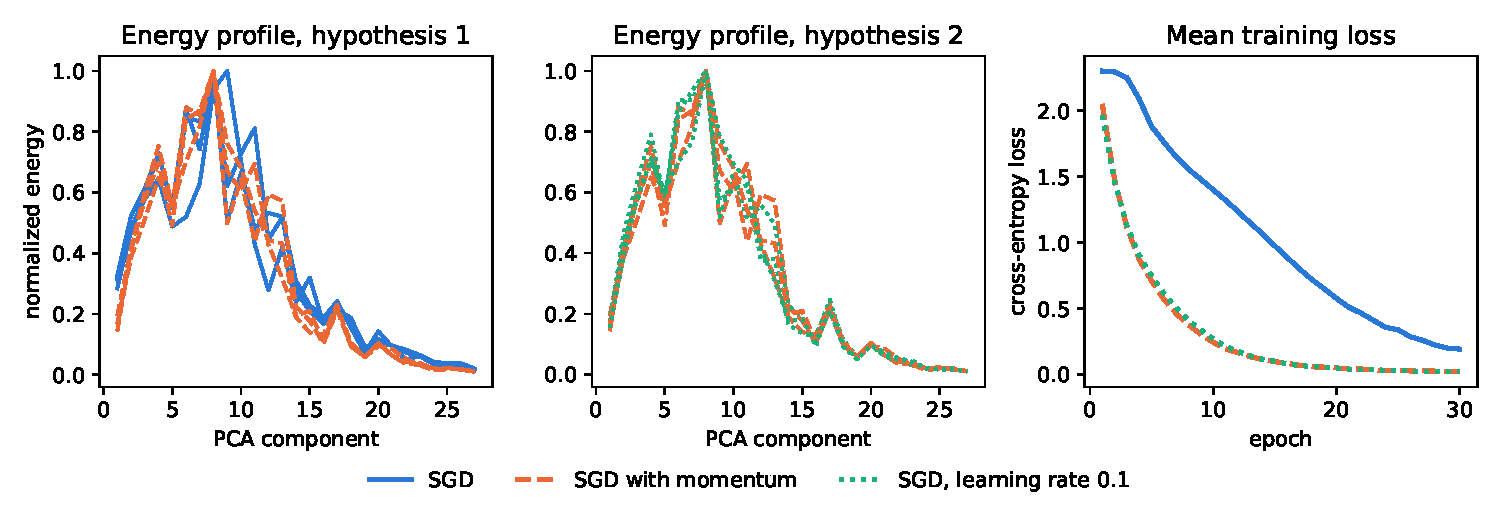
\includegraphics[width=0.9\textwidth]{energy_and_loss_large_lr.pdf}
\caption{First-layer energy profiles, one line per run, and training loss.
The left panel compares plain SGD with momentum (hypothesis 1). The middle
panel compares momentum with plain SGD at learning rate 0.1 (hypothesis 2).
The right panel shows the training loss per epoch, averaged over three seeds.}
\label{fig:energy_and_loss}
\end{figure*}

\subsection{Accuracy}
At learning rate 0.01, momentum has the higher test accuracy on every seed
(Tables~\ref{tab:results} and~\ref{tab:runs}). The gain is 27.34, 25.89, and
18.84 percentage points, with a mean of 24.02. The smallest gain is 3.5 times
the standard deviation of plain SGD across seeds.

\subsection{Training Time}
Plain SGD takes 587.9~s on average and momentum takes 593.6~s, a ratio of
1.01. The difference of 5.7~s is close to the spread across seeds, which is
3.6~s and 4.9~s.

\subsection{Energy Profiles}
Between seeds, the profile correlations of plain SGD are 0.970, 0.887, and
0.900. With momentum they are 0.960, 0.965, and 0.982. On the same seed, the
correlations between plain SGD and momentum are 0.989, 0.983, and 0.950. In
Fig.~\ref{fig:energy_and_loss} (left), five of the six profiles peak at
component 8. The plain SGD run of seed 438 peaks at component 9, and it is
part of the three lowest correlations, 0.887, 0.900, and 0.950.

\subsection{Training Loss}
At epochs 5, 10, and 20 the mean training loss of plain SGD is 1.881, 1.401,
and 0.578, and the loss with momentum is 0.711, 0.245, and 0.051
(Fig.~\ref{fig:energy_and_loss}, right). Plain SGD ends at 0.193 and
momentum ends at 0.022. Momentum passes the final loss of plain SGD at epoch
12.

\subsection{Larger Learning Rate}
Plain SGD with learning rate 0.1 reaches test accuracies of 79.06\%, 63.65\%,
and 75.73\%. The differences from momentum on the same seed are $+1.61$,
$-15.30$, and $-3.55$ points, a mean of $-5.75$. The profile correlations with
the momentum run of the same seed are 0.996, 0.993, and 0.992
(Fig.~\ref{fig:energy_and_loss}, middle). Between seeds they are 0.985, 0.959,
and 0.976. The mean training loss stays within 0.084 of the momentum loss at
every epoch (Fig.~\ref{fig:energy_and_loss}, right). At epochs 5, 10, and 20
it is 0.751, 0.270, and 0.050, and it ends at 0.021.

We trained these runs three times with the same seeds, initial weights, and
batch order, and the tables report the third attempt. The first attempt lost
its files when its session expired, and the second saved an incorrect machine
name. The mean test accuracy was 69.06\%, 73.29\%, and 72.81\%. On seed 436
it was 59.98\%, 72.74\%, and 79.06\%. In all three attempts the profile
correlation with momentum was at least 0.987, and the final training loss was
0.016 to 0.028.

\section{Discussion}
\subsection{Hypothesis 1}
The data support all four parts. With momentum the seed correlations are 0.96
to 0.98 (part 1). On the same seed, the two optimizers have correlations of
0.95 to 0.99 (part 2). Momentum gains 18.84 to 27.34 points of test accuracy
(part 3) and costs 1\% more training time (part 4).

\subsection{Hypothesis 2}
The data support one of the two criteria. Every profile correlation with
momentum is at least 0.992, above the threshold of 0.96. The mean test
accuracy is 5.75 points below momentum, outside the threshold of 2 points. The
two earlier attempts give the same verdict, with means 9.50 and 5.27 points
below momentum. A learning rate 10 times larger reproduces the training loss
and the first-layer profile of momentum, and not its test accuracy.

Momentum reaches the final training loss of plain SGD in 12 of the 30 epochs.
Plain SGD with learning rate 0.1 also takes 12 epochs, and its loss stays
within 0.084 of the momentum loss at every epoch. Momentum 0.9 therefore
trained like a step 10 times larger, the limit of (\ref{eq:momentum}).

\subsection{Comparison with the Original Paper}
Our seed correlation for plain SGD at learning rate 0.01 is 0.92, below the
0.99 in \cite{chowers2023}. Those runs had not converged, with a mean training
loss of 0.193 at epoch 30. The momentum runs and the learning rate 0.1 runs
ended at 0.022 and 0.021, and both groups have a seed correlation of 0.97. By
(\ref{eq:formula}) the profile depends on the step size and the number of
steps, so the lower correlation is consistent with incomplete training.

The results agree with the account in \cite{chowers2023} that the patch
statistics set the profile. Momentum and the learning rate change the size of
each step and leave the data unchanged. Our experiment does not extend
(\ref{eq:formula}) to momentum.

\subsection{Generalization Gap}
All nine runs reach a training accuracy of at least 92.6\%, and their test
accuracy is 50.11\% to 79.28\% (Table~\ref{tab:runs}). The learning rate 0.1
runs match the training loss of momentum, so faster training does not explain
all of the accuracy gain of momentum. Their test accuracy changed by up to
19.08 points between attempts on the same seed. We did not enable
deterministic GPU algorithms, so two runs with the same seed can differ. We
did not identify why the test accuracy of plain SGD varies this much when its
training loss does not.

\subsection{Limitations}
We used three seeds, two learning rates, one momentum value, one model, one
dataset, and 30 epochs. We tuned neither learning rate. We ran each hypothesis
1 run once, so we did not measure how repeatable its test accuracies are. The
hypothesis 2 runs used other sessions, so we compare training time only among
the first six runs.

\subsection{Future Work}
We measured test accuracy once, after epoch 30. Evaluating after every epoch
would show whether the test accuracy of plain SGD is stable late in training.
Repeating the runs on CIFAR-100, where \cite{chowers2023} reports 0.97 between
seeds, would test a second dataset. Fitting (\ref{eq:formula}) to the profiles
and comparing the fitted $t$ would show whether momentum acts like a larger
number of plain gradient steps.

\subsection{Conclusion}
For VGG11-BN on CIFAR-10, momentum 0.9 raised test accuracy by 24.02 points
at 1\% more training time, and the first-layer energy profile kept a
correlation of at least 0.95 with the plain SGD profile. Plain SGD with a
learning rate 10 times larger matched the training loss and the profile of
momentum. Its test accuracy was 5.75 points lower on average and changed by up
to 19.08 points between repeated runs.

\section*{Code Availability}
\noindent Original code:\\
\url{https://github.com/RheaChowers/CNNs-First-Layer}\\
Our code:\\
\url{https://github.com/Markus112105/CS436-FinalProj-Fork}

\begin{thebibliography}{1}

\bibitem{chowers2023}
R. Chowers and Y. Weiss, ``What do CNNs learn in the first layer and why? A
linear systems perspective,'' in \emph{Proc. 40th Int. Conf. Mach. Learn.
(ICML)}, 2023.

\bibitem{sutskever2013}
I. Sutskever, J. Martens, G. Dahl, and G. Hinton, ``On the importance of
initialization and momentum in deep learning,'' in \emph{Proc. 30th Int. Conf.
Mach. Learn. (ICML)}, 2013.

\bibitem{simonyan2015}
K. Simonyan and A. Zisserman, ``Very deep convolutional networks for
large-scale image recognition,'' in \emph{Proc. Int. Conf. Learn. Represent.
(ICLR)}, 2015.

\bibitem{ioffe2015}
S. Ioffe and C. Szegedy, ``Batch normalization: Accelerating deep network
training by reducing internal covariate shift,'' in \emph{Proc. 32nd Int. Conf.
Mach. Learn. (ICML)}, 2015.

\bibitem{krizhevsky2009}
A. Krizhevsky, ``Learning multiple layers of features from tiny images,''
Univ. Toronto, Toronto, ON, Canada, Tech. Rep., 2009.

\bibitem{paszke2019}
A. Paszke \emph{et al.}, ``PyTorch: An imperative style, high-performance deep
learning library,'' in \emph{Adv. Neural Inf. Process. Syst. (NeurIPS)}, 2019.

\bibitem{chen2021}
Y. Chen, ``PyTorch CIFAR models,'' GitHub repository. [Online]. Available:
\url{https://github.com/chenyaofo/pytorch-cifar-models}

\end{thebibliography}

\end{document}
